% tirlnx01 - Materiaal om het keuzevak Linux te geven 
% op de Hogeschool Rotterdam.
% Copyright (C) 2010 - 2011  Paul Sohier, Kevin van der Vlist
%
% This program is free software: you can redistribute it and/or modify
% it under the terms of the GNU General Public License as published by
% the Free Software Foundation, either version 3 of the License, or
% (at your option) any later version.
%
% This program is distributed in the hope that it will be useful,
% but WITHOUT ANY WARRANTY; without even the implied warranty of
% MERCHANTABILITY or FITNESS FOR A PARTICULAR PURPOSE.  See the
% GNU General Public License for more details.
%
% You should have received a copy of the GNU General Public License
% along with this program.  If not, see <http://www.gnu.org/licenses/>.
%
% Kevin van der Vlist - kevin@kevinvandervlist.nl
% Paul Sohier - paul@paulsohier.nl

\chapter{X}
Om op een \emph{Linux} systeem gebruik te kunnen maken van een grafische omgeving is het \emph{X framework} ontwikkeld. Het is een product wat wordt geleid door de \emph{X.Org Foundation}. 

\section{Geschiedenis}
De \emph{X.Org foundation} is ontstaan uit een samenwerkingsverband tussen de organisatie die de \emph{X} standaarden regelt en een groep vroegere ontwikkelaars van het \emph{XFree86} project. 

De reden dat deze ontwikkelaars zijn overgestapt naar de \emph{X.Org foundation} is een ruzie over het nieuwe licentiemodel van \emph{XFree86}. Er heeft daarom een \emph{fork} plaatsgevonden waarna het project \emph{X11} werd ondergebracht bij de \emph{X.Org foundation}. 

\section{Implementatie}
De basis van het \emph{X} protocol is in de jaren 80 ontwikkeld. De bedoeling was om een generiek \emph{client-server} model te hebben om grafische toepassingen te gebruiken. Er moest op een willekeurige machine een applicatie gedraaid moeten worden, die gebruikt kon worden op een willekeurige andere machine. De keuze van het platform zou dit niet mogen belemmeren. 

Er zijn binnen het \emph{X} protocol twee partijen. Deze hebben allebij een eigen taak. 

\subsection{X server}
De \emph{X server} verzorgt de faciliteiten om de verschillende \emph{X clients} te kunnen laten communiceren. Ook biedt het een \emph{display} aan. Dit betekend dus dat er op een \emph{client} een \textbf{\emph{X server}} draait. 

\subsection{X client}
De \emph{X client} zal de diensten van de \emph{X server} gebruiken. De applicaties zelf zijn dus effectief de \textbf{\emph{X clients}}. Als er op een applicatie een grafisch programma wordt gestart zal dit dus een \emph{client} zijn naar de \emph{X server} van de verbonden gebruiker. 

\subsection{Protocol}
Voor de communicatie tussen de \emph{X} server en de \emph{X} client is er gekozen voor een compleet transparant protocol. Het is niet afhankelijk van het medium waar het transport over plaatsvindt, waardoor gebruikers ook via het netwerk software kunnen gebruiken. 

\subsection{Communicatie}
Wanneer alle bovenstaande aspecten bij elkaar worden gevoegd zal er het volgende totaalbeeld uit komen, zie figuur \ref{fig:xs2}:
% Plaatje niet nodig, leg in een keer 2 uit. Als het toch nodig is, hij blijft in de sources
%\begin{figure}[h]%Dit plaatje is overbodig
%  \begin{center}
%    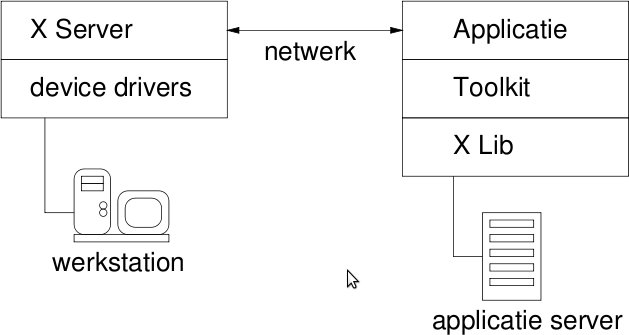
\includegraphics[scale=0.4]{images/xserver}
%  \end{center}
%  \caption{X client/server overzicht}
%  \label{fig:xs}
%\end{figure}

\begin{figure}[h]
  \begin{center}
    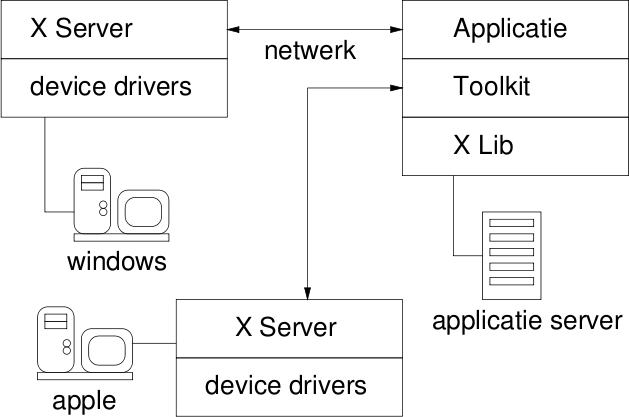
\includegraphics[scale=0.4]{images/xserver2}
  \end{center}
  \caption{X client/server overzicht}
  \label{fig:xs2}
\end{figure}
Hier is duidelijk te zien hoe de verschillende onderdelen van \emph{X} met elkaar samenwerken. Een applicatie gestart op een applicatie server is generiek. Deze zal verbinding maken met de \emph{X server} van de \emph{client}, welke de hardware-specifieke zaken regelt. Om deze reden zal de ``Apple'' computer dus een andere \emph{X server} hebben dan de ``Windows'' computer. 

\section{Window Manager}
Een \emph{window manager} is een pakket wat alle zaken regelt die gerelateerd zijn aan het venster beheer. Denk hierbij bijvoorbeeld aan de mogelijkheid om vensters te verslepen of van grootte te veranderen. De meeste \emph{window managers} zullen ook voor een \emph{desktop} omgeving zorgen, waardoor het paketten zijn die sterk zijn ge\"{i}ntegreerd met basis \emph{desktop} applicaties. 

De bekendste toepassing die een \emph{window manager} uitvoert is het \emph{reparenten} van een scherm. Hier wordt er nog een extra ``venster'' om een programma heen gezet, welke vaak bestaat uit de titelbalk. Dit kan dan bijvoorbeeld worden gebruikt om vensters te verslepen. 

\section{Installatie}
Op \emph{Slackware} zijn er ook \emph{packages} van \emph{Xorg beschikbaar}. Het installeren hiervan is dan ook relatief eenvoudig. 

Er kan gekozen worden om de volledige \emph{X} suite te installeren, of om de minimale delen ervan te kiezen. Omdat het iets gemakkelijker is om de complete \emph{X} suite te installeren zal dat worden gehanteerd in het onderstaande voorbeeld. 
\begin{lstlisting}
kevin@slackbak:/tmp$ mkdir x
kevin@slackbak:/tmp$ cd x; wget -r -A txz -nd ftp://ftp.fu-berlin.de/unix/linux/mirrors/slackware/slackware-13.1/slackware/x/
[...]
FINISHED --2010-12-15 17:55:16--
Downloaded: 299 files, 84M in 9m 34s (150 KB/s)
kevin@slackbak:/tmp/x$ su
Password: 
root@slackbak:/tmp/x$ installpkg *
\end{lstlisting}%$
Kies als \emph{url} natuurlijk een \emph{mirror} naar keuze uit. Als \texttt{installpkg}\index{installpkg} klaar is zal de basis \emph{X} omgeving ge\"{i}nstalleerd zijn. 

\subsection{KDE}
Er zijn verschillende \emph{window managers} beschikbaar, maar in dit voorbeeld zal \emph{KDE} worden geinstalleerd. Deze \emph{window manager} is ook weer in de \emph{Slackware} repositories te vinden, waardoor het erg gemakkelijk is om op het systeem te zetten. De installatie gaat als volgt:
\begin{lstlisting}
kevin@slackbak:/tmp$ mkdir kde
kevin@slackbak:/tmp$ cd kde; wget -r -A txz -nd ftp://ftp.fu-berlin.de/unix/linux/mirrors/slackware/slackware-13.1/slackware/kde/
[...]
FINISHED --2010-12-15 13:06:36--
Downloaded: 35 files, 374M in 6m 4s (1,03 MB/s)
kevin@slackbak:/tmp/kde$ su
Password: 
root@slackbak:/tmp/kde$ installpkg *
\end{lstlisting}

\subsection{Fluxbox}
Mocht \emph{KDE} te groot bevonden worden kan er ook naar de veel minimalistischere, maar lichtere desktop omgeving is \emph{Fluxbox} gekeken worden. Ook deze is gemakkelijk in gebruik, maar ontzettend flexibel in de configuratie. De installatie gaat als volgt:
\begin{lstlisting}
kevin@slackbak:/tmp$ mkdir fluxbox
kevin@slackbak:/tmp$ cd fluxbox; wget ftp://ftp.fu-berlin.de/unix/linux/mirrors/slackware/slackware-13.1/slackware/xap/fluxbox-1.1.1-i486-2.txz
[...]
2010-12-18 13:27:57 (392 KB/s) - “fluxbox-1.1.1-i486-2.txz” saved [654388]
kevin@slackbak:/tmp/fluxbox$ su
Password: 
root@slackbak:/tmp/fluxbox$ installpkg fluxbox-1.1.1-i486-2.txz
\end{lstlisting}

\section{X configureren}
Moderne implementaties van \emph{X} hebben autodetectie mogelijkheden aan boord. Dit betekend dat het veel eenvoudiger is geworden om \emph{X} te configureren, er hoeft nu niets meer te worden gedaan. 

Mocht het gewenst zijn om een configuratie bestand te genereren, zodat er speciefieke \emph{X} instellingen toegepast kunnen worden. Om een basis configuratie bestand te genereren is het mogelijk gebruik te maken van \texttt{xorgsetup}\index{xorgsetup}. Dit is dus een optionele stap.

\begin{lstlisting}
root@slackbak:/$ xorgsetup
\end{lstlisting}%$

De volgende stap is het opgeven van de \emph{window manager}. Dit kan met het commando \texttt{xwmconfig}\index{xwmconfig}: 

\begin{lstlisting}
kevin@slackbak:$ xwmconfig
\end{lstlisting}%$

\section{X Starten}
\emph{X} kan nu gestart worden doort het commando \texttt{startx}\index{startx} uit te voeren. 

\section{Remote X}
Aangezien het \emph{X11} framework dus de mogelijkheid biedt om applicaties remote te draaien zal er enige uitleg volgen over hoe dit is uit te voeren. 

De gemakkelijkste manier is om een \emph{ssh} verbinding te openen met \emph{X forwarding}. Dit kan erg simpel met het programma \texttt{ssh}\index{ssh}:
\begin{lstlisting}
kevin@slackbak:~$ ssh -XY host.nl
\end{lstlisting}%$
De ``-X'' optie zorgt ervoor dat er aan \emph{X forwarding} gedaan kan worden, met ``-Y'' wordt gezegd dat de \emph{X11} verbinding te vertrouwen is. Door de laatste optie hoeven er geen specifieke beveiligings opties te worden toegepast, waardoor het erg eenvoudig in gebruik is. 

Deze optie vereist wel dat de \emph{SSH server} deze mogelijkheden ondersteund. In het onderstaande voorbeeld is dit het geval:
\begin{lstlisting}
kevin@slackbak:~$ grep "X11Forwarding" /etc/ssh/sshd_config 
X11Forwarding yes
\end{lstlisting}%$
